% Generated by misc/paper_b/tools/build_figures.py from NUMBERS_TABLE.csv. Do not edit.
% Own effects of the six sign bits, trained vs prompted (full 7 x 6 matrix is not banked)
\documentclass[border=3pt]{standalone}
\usepackage[T1]{fontenc}
\usepackage{lmodern,amsmath,xcolor}
\usepackage{tikz}
\pdftrailerid{}
\definecolor{cA}{HTML}{0072B2}% blue
\definecolor{cB}{HTML}{D55E00}% vermillion
\definecolor{cC}{HTML}{009E73}% green
\definecolor{cD}{HTML}{CC79A7}% purple
\definecolor{cG}{HTML}{6B6B6B}% grey
\definecolor{cS}{HTML}{3A3A3A}
\definecolor{zebra}{HTML}{F1F1F1}
\definecolor{gridc}{HTML}{C8C8C8}
\newcommand{\Px}{0}\newcommand{\Pmin}{0}\newcommand{\Psc}{1}
% \setpanel{x0 cm}{data value at x0}{cm per data unit}: every data x below is x0 + (v - vmin) * scale.
\newcommand{\setpanel}[3]{\renewcommand{\Px}{#1}\renewcommand{\Pmin}{#2}\renewcommand{\Psc}{#3}}
\newcommand{\XX}[1]{\fpeval{\Px+((#1)-(\Pmin))*\Psc}}
% markers: o filled circle, s filled square, d hollow diamond, t filled triangle, h hollow circle, q hollow square
\newcommand{\mk}[4]{% style colour x y
  \ifx#1o\fill[#2] (#3,#4) circle (0.095);\fi
  \ifx#1h\draw[#2,fill=white,line width=0.7pt] (#3,#4) circle (0.095);\fi
  \ifx#1s\fill[#2] (#3-0.088,#4-0.088) rectangle (#3+0.088,#4+0.088);\fi
  \ifx#1q\draw[#2,fill=white,line width=0.7pt] (#3-0.085,#4-0.085) rectangle (#3+0.085,#4+0.085);\fi
  \ifx#1d\draw[#2,fill=white,line width=0.7pt] (#3,#4+0.125)--(#3+0.125,#4)--(#3,#4-0.125)--(#3-0.125,#4)--cycle;\fi
  \ifx#1t\fill[#2] (#3,#4+0.115)--(#3+0.105,#4-0.085)--(#3-0.105,#4-0.085)--cycle;\fi}
% interval with point: claim, lo, value, hi, y, style, colour, dash(solid|dashed)
\newcommand{\ival}[8]{%
  \edef\xl{\XX{#2}}\edef\xv{\XX{#3}}\edef\xh{\XX{#4}}%
  \draw[#7,line width=0.8pt,#8] (\xl,#5)--(\xh,#5);
  \draw[#7,line width=0.8pt] (\xl,#5-0.055)--(\xl,#5+0.055);
  \draw[#7,line width=0.8pt] (\xh,#5-0.055)--(\xh,#5+0.055);
  \mk{#6}{#7}{\xv}{#5}}
% point only
\newcommand{\pval}[5]{\edef\xv{\XX{#2}}\mk{#4}{#5}{\xv}{#3}}
% stem from the panel zero to the value, with marker: claim, value, y, style, colour
\newcommand{\lval}[5]{\edef\xv{\XX{#2}}\edef\xz{\XX{0}}%
  \draw[#5,line width=0.8pt] (\xz,#3)--(\xv,#3);\mk{#4}{#5}{\xv}{#3}}
% vertical reference line at a data value: claim, value, y0, y1, colour
\newcommand{\vref}[5]{\edef\xv{\XX{#2}}\draw[#5,dashed,line width=0.8pt] (\xv,#3)--(\xv,#4);}
% a printed number tied to a table cell: claim, field, printed, prefix, suffix, x, y, anchor, background fill
\newcommand{\lbl}[9]{\node[anchor=#8,fill=#9,inner sep=1pt,font=\footnotesize] at (#6,#7) {#4#3#5};}
% a printed value with its interval: claim, printed value, printed lo, printed hi, x, y, anchor
\newcommand{\lblci}[7]{\node[anchor=#7,inner sep=0pt,font=\footnotesize] at (#5,#6) {#2\,[#3, #4]};}
% free text (no data)
\newcommand{\txt}[4]{\node[anchor=#3,inner sep=0pt,font=#4] at (#1) {#2};}
\begin{document}
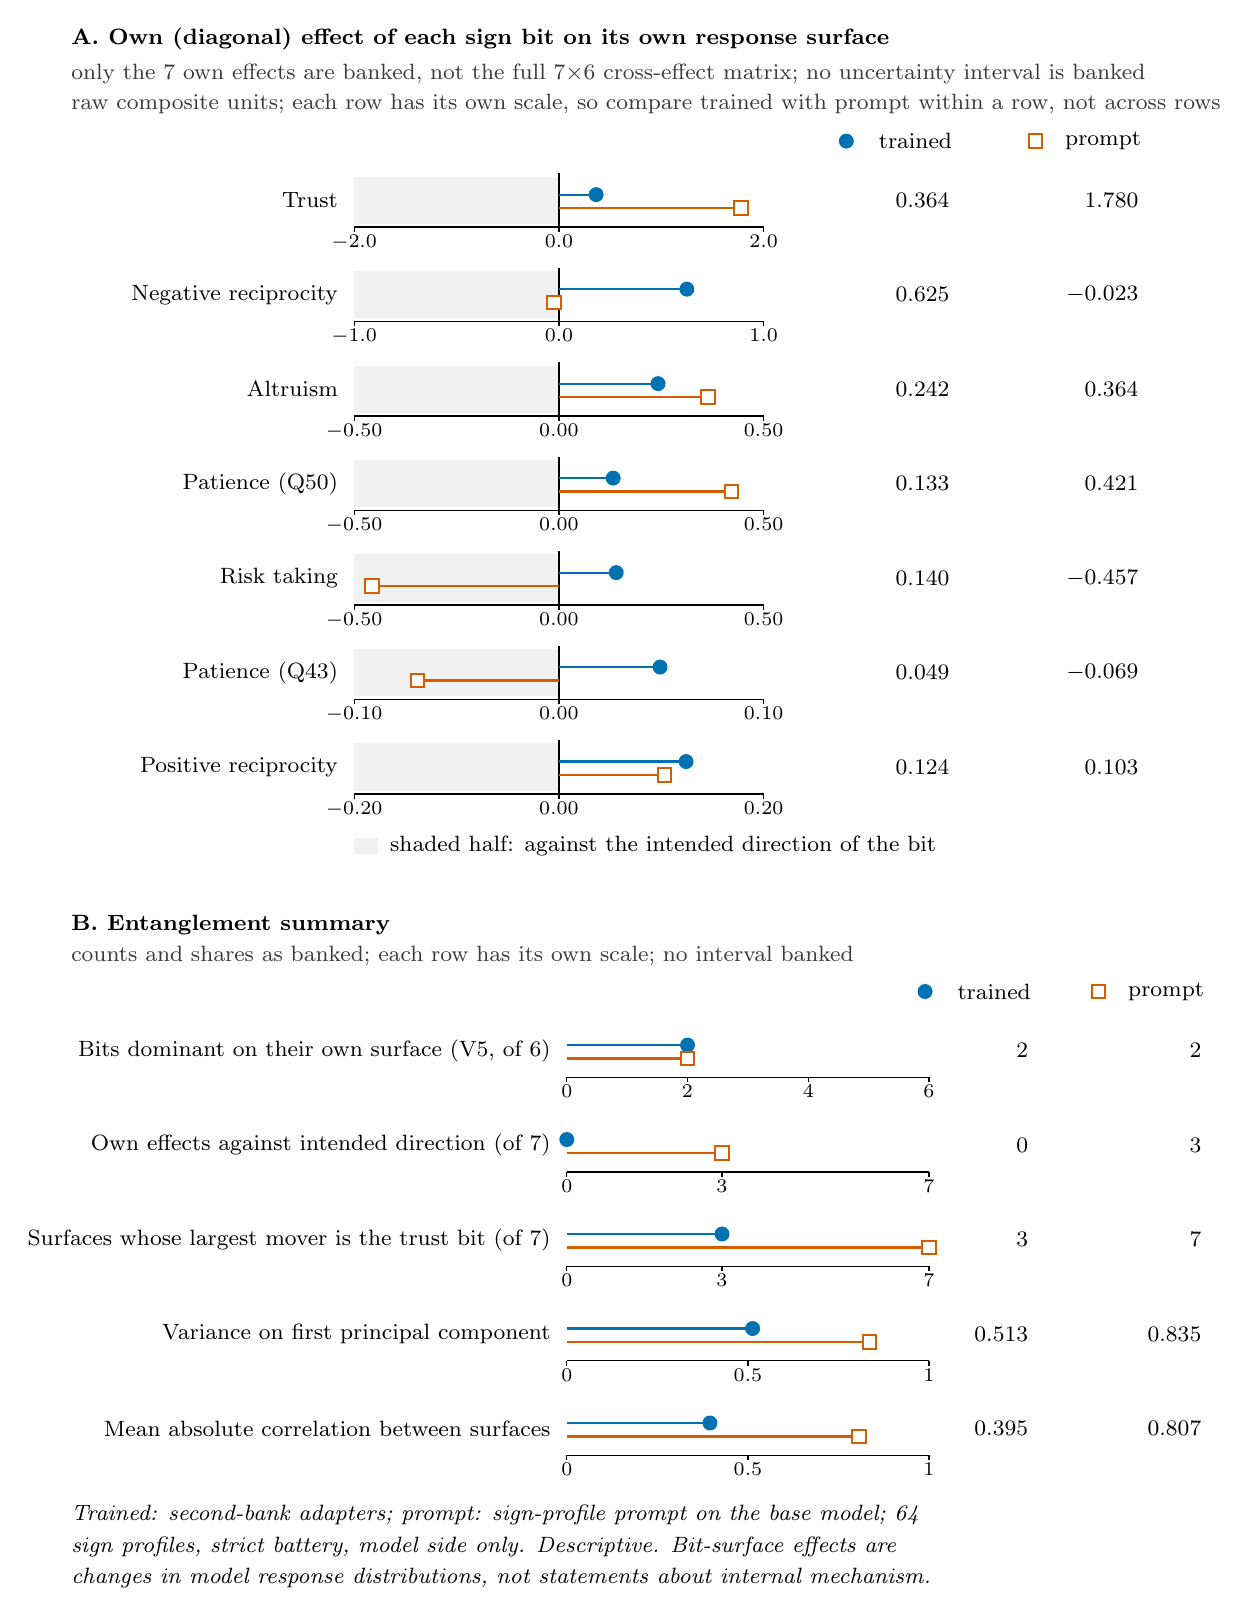
\begin{tikzpicture}[x=1cm,y=1cm,every node/.style={text=black}]
\txt{0.000,1.550}{\textbf{A. Own (diagonal) effect of each sign bit on its own response surface}}{west}{\footnotesize}
\txt{0.000,1.100}{\footnotesize\textcolor{cS}{only the 7 own effects are banked, not the full 7$\times$6 cross-effect matrix; no uncertainty interval is banked}}{west}{\footnotesize}
\txt{0.000,0.720}{\footnotesize\textcolor{cS}{raw composite units; each row has its own scale, so compare trained with prompt within a row, not across rows}}{west}{\footnotesize}
\mk{o}{cA}{9.85}{0.250}
\txt{11.200,0.250}{trained}{east}{\footnotesize}
\mk{q}{cB}{12.25}{0.250}
\txt{13.600,0.250}{prompt}{east}{\footnotesize}
\setpanel{3.600000000000000088817841970012523233890533447265625}{-2}{1.300000}
\fill[zebra] (3.600,-0.800) rectangle (6.200,-0.200);
\draw[black,line width=0.9pt] (6.200,-0.840)--(6.200,-0.160);
\draw[black,line width=0.5pt] (3.600,-0.840)--(8.800,-0.840);
\draw[black,line width=0.5pt] (3.600,-0.840)--(3.600,-0.900);
\node[anchor=north,inner sep=1pt,font=\scriptsize] at (3.600,-0.900) {$-$2.0};
\draw[black,line width=0.5pt] (6.200,-0.840)--(6.200,-0.900);
\node[anchor=north,inner sep=1pt,font=\scriptsize] at (6.200,-0.900) {0.0};
\draw[black,line width=0.5pt] (8.800,-0.840)--(8.800,-0.900);
\node[anchor=north,inner sep=1pt,font=\scriptsize] at (8.800,-0.900) {2.0};
\txt{3.400,-0.500}{Trust}{east}{\footnotesize}
\setpanel{3.600000000000000088817841970012523233890533447265625}{-2}{1.300000}
\lval{FX_adapter64_trust_own_beta}{0.36358243388594513}{-0.430}{o}{cA}
\setpanel{3.600000000000000088817841970012523233890533447265625}{-2}{1.300000}
\lval{FX_signprompt64_trust_own_beta}{1.7796863115995532}{-0.600}{q}{cB}
\lbl{FX_adapter64_trust_own_beta}{value}{0.364}{}{}{11.200}{-0.500}{east}{none}
\lbl{FX_signprompt64_trust_own_beta}{value}{1.780}{}{}{13.600}{-0.500}{east}{none}
\setpanel{3.600000000000000088817841970012523233890533447265625}{-1}{2.600000}
\fill[zebra] (3.600,-2.000) rectangle (6.200,-1.400);
\draw[black,line width=0.9pt] (6.200,-2.040)--(6.200,-1.360);
\draw[black,line width=0.5pt] (3.600,-2.040)--(8.800,-2.040);
\draw[black,line width=0.5pt] (3.600,-2.040)--(3.600,-2.100);
\node[anchor=north,inner sep=1pt,font=\scriptsize] at (3.600,-2.100) {$-$1.0};
\draw[black,line width=0.5pt] (6.200,-2.040)--(6.200,-2.100);
\node[anchor=north,inner sep=1pt,font=\scriptsize] at (6.200,-2.100) {0.0};
\draw[black,line width=0.5pt] (8.800,-2.040)--(8.800,-2.100);
\node[anchor=north,inner sep=1pt,font=\scriptsize] at (8.800,-2.100) {1.0};
\txt{3.400,-1.700}{Negative reciprocity}{east}{\footnotesize}
\setpanel{3.600000000000000088817841970012523233890533447265625}{-1}{2.600000}
\lval{FX_adapter64_negrecip_own_beta}{0.6247672859863043}{-1.630}{o}{cA}
\setpanel{3.600000000000000088817841970012523233890533447265625}{-1}{2.600000}
\lval{FX_signprompt64_negrecip_own_beta}{-0.023307224836190077}{-1.800}{q}{cB}
\lbl{FX_adapter64_negrecip_own_beta}{value}{0.625}{}{}{11.200}{-1.700}{east}{none}
\lbl{FX_signprompt64_negrecip_own_beta}{value}{$-$0.023}{}{}{13.600}{-1.700}{east}{none}
\setpanel{3.600000000000000088817841970012523233890533447265625}{-0.5}{5.200000}
\fill[zebra] (3.600,-3.200) rectangle (6.200,-2.600);
\draw[black,line width=0.9pt] (6.200,-3.240)--(6.200,-2.560);
\draw[black,line width=0.5pt] (3.600,-3.240)--(8.800,-3.240);
\draw[black,line width=0.5pt] (3.600,-3.240)--(3.600,-3.300);
\node[anchor=north,inner sep=1pt,font=\scriptsize] at (3.600,-3.300) {$-$0.50};
\draw[black,line width=0.5pt] (6.200,-3.240)--(6.200,-3.300);
\node[anchor=north,inner sep=1pt,font=\scriptsize] at (6.200,-3.300) {0.00};
\draw[black,line width=0.5pt] (8.800,-3.240)--(8.800,-3.300);
\node[anchor=north,inner sep=1pt,font=\scriptsize] at (8.800,-3.300) {0.50};
\txt{3.400,-2.900}{Altruism}{east}{\footnotesize}
\setpanel{3.600000000000000088817841970012523233890533447265625}{-0.5}{5.200000}
\lval{FX_adapter64_altruism_own_beta}{0.24208090186424142}{-2.830}{o}{cA}
\setpanel{3.600000000000000088817841970012523233890533447265625}{-0.5}{5.200000}
\lval{FX_signprompt64_altruism_own_beta}{0.3643732082194353}{-3.000}{q}{cB}
\lbl{FX_adapter64_altruism_own_beta}{value}{0.242}{}{}{11.200}{-2.900}{east}{none}
\lbl{FX_signprompt64_altruism_own_beta}{value}{0.364}{}{}{13.600}{-2.900}{east}{none}
\setpanel{3.600000000000000088817841970012523233890533447265625}{-0.5}{5.200000}
\fill[zebra] (3.600,-4.400) rectangle (6.200,-3.800);
\draw[black,line width=0.9pt] (6.200,-4.440)--(6.200,-3.760);
\draw[black,line width=0.5pt] (3.600,-4.440)--(8.800,-4.440);
\draw[black,line width=0.5pt] (3.600,-4.440)--(3.600,-4.500);
\node[anchor=north,inner sep=1pt,font=\scriptsize] at (3.600,-4.500) {$-$0.50};
\draw[black,line width=0.5pt] (6.200,-4.440)--(6.200,-4.500);
\node[anchor=north,inner sep=1pt,font=\scriptsize] at (6.200,-4.500) {0.00};
\draw[black,line width=0.5pt] (8.800,-4.440)--(8.800,-4.500);
\node[anchor=north,inner sep=1pt,font=\scriptsize] at (8.800,-4.500) {0.50};
\txt{3.400,-4.100}{Patience (Q50)}{east}{\footnotesize}
\setpanel{3.600000000000000088817841970012523233890533447265625}{-0.5}{5.200000}
\lval{FX_adapter64_patience_Q50_own_beta}{0.13250479634657153}{-4.030}{o}{cA}
\setpanel{3.600000000000000088817841970012523233890533447265625}{-0.5}{5.200000}
\lval{FX_signprompt64_patience_Q50_own_beta}{0.4210699711397531}{-4.200}{q}{cB}
\lbl{FX_adapter64_patience_Q50_own_beta}{value}{0.133}{}{}{11.200}{-4.100}{east}{none}
\lbl{FX_signprompt64_patience_Q50_own_beta}{value}{0.421}{}{}{13.600}{-4.100}{east}{none}
\setpanel{3.600000000000000088817841970012523233890533447265625}{-0.5}{5.200000}
\fill[zebra] (3.600,-5.600) rectangle (6.200,-5.000);
\draw[black,line width=0.9pt] (6.200,-5.640)--(6.200,-4.960);
\draw[black,line width=0.5pt] (3.600,-5.640)--(8.800,-5.640);
\draw[black,line width=0.5pt] (3.600,-5.640)--(3.600,-5.700);
\node[anchor=north,inner sep=1pt,font=\scriptsize] at (3.600,-5.700) {$-$0.50};
\draw[black,line width=0.5pt] (6.200,-5.640)--(6.200,-5.700);
\node[anchor=north,inner sep=1pt,font=\scriptsize] at (6.200,-5.700) {0.00};
\draw[black,line width=0.5pt] (8.800,-5.640)--(8.800,-5.700);
\node[anchor=north,inner sep=1pt,font=\scriptsize] at (8.800,-5.700) {0.50};
\txt{3.400,-5.300}{Risk taking}{east}{\footnotesize}
\setpanel{3.600000000000000088817841970012523233890533447265625}{-0.5}{5.200000}
\lval{FX_adapter64_risktaking_own_beta}{0.14000873839053002}{-5.230}{o}{cA}
\setpanel{3.600000000000000088817841970012523233890533447265625}{-0.5}{5.200000}
\lval{FX_signprompt64_risktaking_own_beta}{-0.4567087152154239}{-5.400}{q}{cB}
\lbl{FX_adapter64_risktaking_own_beta}{value}{0.140}{}{}{11.200}{-5.300}{east}{none}
\lbl{FX_signprompt64_risktaking_own_beta}{value}{$-$0.457}{}{}{13.600}{-5.300}{east}{none}
\setpanel{3.600000000000000088817841970012523233890533447265625}{-0.1}{26.000000}
\fill[zebra] (3.600,-6.800) rectangle (6.200,-6.200);
\draw[black,line width=0.9pt] (6.200,-6.840)--(6.200,-6.160);
\draw[black,line width=0.5pt] (3.600,-6.840)--(8.800,-6.840);
\draw[black,line width=0.5pt] (3.600,-6.840)--(3.600,-6.900);
\node[anchor=north,inner sep=1pt,font=\scriptsize] at (3.600,-6.900) {$-$0.10};
\draw[black,line width=0.5pt] (6.200,-6.840)--(6.200,-6.900);
\node[anchor=north,inner sep=1pt,font=\scriptsize] at (6.200,-6.900) {0.00};
\draw[black,line width=0.5pt] (8.800,-6.840)--(8.800,-6.900);
\node[anchor=north,inner sep=1pt,font=\scriptsize] at (8.800,-6.900) {0.10};
\txt{3.400,-6.500}{Patience (Q43)}{east}{\footnotesize}
\setpanel{3.600000000000000088817841970012523233890533447265625}{-0.1}{26.000000}
\lval{FX_adapter64_patience_Q43_own_beta}{0.049414495561863836}{-6.430}{o}{cA}
\setpanel{3.600000000000000088817841970012523233890533447265625}{-0.1}{26.000000}
\lval{FX_signprompt64_patience_Q43_own_beta}{-0.06918062400906969}{-6.600}{q}{cB}
\lbl{FX_adapter64_patience_Q43_own_beta}{value}{0.049}{}{}{11.200}{-6.500}{east}{none}
\lbl{FX_signprompt64_patience_Q43_own_beta}{value}{$-$0.069}{}{}{13.600}{-6.500}{east}{none}
\setpanel{3.600000000000000088817841970012523233890533447265625}{-0.2}{13.000000}
\fill[zebra] (3.600,-8.000) rectangle (6.200,-7.400);
\draw[black,line width=0.9pt] (6.200,-8.040)--(6.200,-7.360);
\draw[black,line width=0.5pt] (3.600,-8.040)--(8.800,-8.040);
\draw[black,line width=0.5pt] (3.600,-8.040)--(3.600,-8.100);
\node[anchor=north,inner sep=1pt,font=\scriptsize] at (3.600,-8.100) {$-$0.20};
\draw[black,line width=0.5pt] (6.200,-8.040)--(6.200,-8.100);
\node[anchor=north,inner sep=1pt,font=\scriptsize] at (6.200,-8.100) {0.00};
\draw[black,line width=0.5pt] (8.800,-8.040)--(8.800,-8.100);
\node[anchor=north,inner sep=1pt,font=\scriptsize] at (8.800,-8.100) {0.20};
\txt{3.400,-7.700}{Positive reciprocity}{east}{\footnotesize}
\setpanel{3.600000000000000088817841970012523233890533447265625}{-0.2}{13.000000}
\lval{FX_adapter64_posrecip_own_beta}{0.12419389655920332}{-7.630}{o}{cA}
\setpanel{3.600000000000000088817841970012523233890533447265625}{-0.2}{13.000000}
\lval{FX_signprompt64_posrecip_own_beta}{0.10313613448686443}{-7.800}{q}{cB}
\lbl{FX_adapter64_posrecip_own_beta}{value}{0.124}{}{}{11.200}{-7.700}{east}{none}
\lbl{FX_signprompt64_posrecip_own_beta}{value}{0.103}{}{}{13.600}{-7.700}{east}{none}
\fill[zebra] (3.6,-8.800) rectangle (3.9,-8.600);
\txt{4.050,-8.700}{shaded half: against the intended direction of the bit}{west}{\footnotesize}
\txt{0.000,-9.700}{\textbf{B. Entanglement summary}}{west}{\footnotesize}
\txt{0.000,-10.100}{\footnotesize\textcolor{cS}{counts and shares as banked; each row has its own scale; no interval banked}}{west}{\footnotesize}
\mk{o}{cA}{10.85}{-10.550}
\txt{12.200,-10.550}{trained}{east}{\footnotesize}
\mk{q}{cB}{13.05}{-10.550}
\txt{14.400,-10.550}{prompt}{east}{\footnotesize}
\setpanel{6.29999999999999982236431605997495353221893310546875}{0}{0.766667}
\draw[black,line width=0.5pt] (6.300,-11.640)--(10.900,-11.640);
\draw[black,line width=0.5pt] (6.300,-11.640)--(6.300,-11.700);
\node[anchor=north,inner sep=1pt,font=\scriptsize] at (6.300,-11.700) {0};
\draw[black,line width=0.5pt] (7.833,-11.640)--(7.833,-11.700);
\node[anchor=north,inner sep=1pt,font=\scriptsize] at (7.833,-11.700) {2};
\draw[black,line width=0.5pt] (9.367,-11.640)--(9.367,-11.700);
\node[anchor=north,inner sep=1pt,font=\scriptsize] at (9.367,-11.700) {4};
\draw[black,line width=0.5pt] (10.900,-11.640)--(10.900,-11.700);
\node[anchor=north,inner sep=1pt,font=\scriptsize] at (10.900,-11.700) {6};
\txt{6.100,-11.300}{Bits dominant on their own surface (V5, of 6)}{east}{\footnotesize}
\setpanel{6.29999999999999982236431605997495353221893310546875}{0}{0.766667}
\lval{FX_adapter64_V5_hits}{2}{-11.230}{o}{cA}
\setpanel{6.29999999999999982236431605997495353221893310546875}{0}{0.766667}
\lval{FX_signprompt64_V5_hits}{2}{-11.400}{q}{cB}
\lbl{FX_adapter64_V5_hits}{value}{2}{}{}{12.200}{-11.300}{east}{none}
\lbl{FX_signprompt64_V5_hits}{value}{2}{}{}{14.400}{-11.300}{east}{none}
\setpanel{6.29999999999999982236431605997495353221893310546875}{0}{0.657143}
\draw[black,line width=0.5pt] (6.300,-12.840)--(10.900,-12.840);
\draw[black,line width=0.5pt] (6.300,-12.840)--(6.300,-12.900);
\node[anchor=north,inner sep=1pt,font=\scriptsize] at (6.300,-12.900) {0};
\draw[black,line width=0.5pt] (8.271,-12.840)--(8.271,-12.900);
\node[anchor=north,inner sep=1pt,font=\scriptsize] at (8.271,-12.900) {3};
\draw[black,line width=0.5pt] (10.900,-12.840)--(10.900,-12.900);
\node[anchor=north,inner sep=1pt,font=\scriptsize] at (10.900,-12.900) {7};
\txt{6.100,-12.500}{Own effects against intended direction (of 7)}{east}{\footnotesize}
\setpanel{6.29999999999999982236431605997495353221893310546875}{0}{0.657143}
\lval{FX_adapter64_own_effects_wrong_signed}{0}{-12.430}{o}{cA}
\setpanel{6.29999999999999982236431605997495353221893310546875}{0}{0.657143}
\lval{FX_signprompt64_own_effects_wrong_signed}{3}{-12.600}{q}{cB}
\lbl{FX_adapter64_own_effects_wrong_signed}{value}{0}{}{}{12.200}{-12.500}{east}{none}
\lbl{FX_signprompt64_own_effects_wrong_signed}{value}{3}{}{}{14.400}{-12.500}{east}{none}
\setpanel{6.29999999999999982236431605997495353221893310546875}{0}{0.657143}
\draw[black,line width=0.5pt] (6.300,-14.040)--(10.900,-14.040);
\draw[black,line width=0.5pt] (6.300,-14.040)--(6.300,-14.100);
\node[anchor=north,inner sep=1pt,font=\scriptsize] at (6.300,-14.100) {0};
\draw[black,line width=0.5pt] (8.271,-14.040)--(8.271,-14.100);
\node[anchor=north,inner sep=1pt,font=\scriptsize] at (8.271,-14.100) {3};
\draw[black,line width=0.5pt] (10.900,-14.040)--(10.900,-14.100);
\node[anchor=north,inner sep=1pt,font=\scriptsize] at (10.900,-14.100) {7};
\txt{6.100,-13.700}{Surfaces whose largest mover is the trust bit (of 7)}{east}{\footnotesize}
\setpanel{6.29999999999999982236431605997495353221893310546875}{0}{0.657143}
\lval{FX_adapter64_surfaces_largest_mover_is_trust_bit}{3}{-13.630}{o}{cA}
\setpanel{6.29999999999999982236431605997495353221893310546875}{0}{0.657143}
\lval{FX_signprompt64_surfaces_largest_mover_is_trust_bit}{7}{-13.800}{q}{cB}
\lbl{FX_adapter64_surfaces_largest_mover_is_trust_bit}{value}{3}{}{}{12.200}{-13.700}{east}{none}
\lbl{FX_signprompt64_surfaces_largest_mover_is_trust_bit}{value}{7}{}{}{14.400}{-13.700}{east}{none}
\setpanel{6.29999999999999982236431605997495353221893310546875}{0}{4.600000}
\draw[black,line width=0.5pt] (6.300,-15.240)--(10.900,-15.240);
\draw[black,line width=0.5pt] (6.300,-15.240)--(6.300,-15.300);
\node[anchor=north,inner sep=1pt,font=\scriptsize] at (6.300,-15.300) {0};
\draw[black,line width=0.5pt] (8.600,-15.240)--(8.600,-15.300);
\node[anchor=north,inner sep=1pt,font=\scriptsize] at (8.600,-15.300) {0.5};
\draw[black,line width=0.5pt] (10.900,-15.240)--(10.900,-15.300);
\node[anchor=north,inner sep=1pt,font=\scriptsize] at (10.900,-15.300) {1};
\txt{6.100,-14.900}{Variance on first principal component}{east}{\footnotesize}
\setpanel{6.29999999999999982236431605997495353221893310546875}{0}{4.600000}
\lval{FX_adapter64_pc1_share}{0.5130116356330489}{-14.830}{o}{cA}
\setpanel{6.29999999999999982236431605997495353221893310546875}{0}{4.600000}
\lval{FX_signprompt64_pc1_share}{0.8352930408769921}{-15.000}{q}{cB}
\lbl{FX_adapter64_pc1_share}{value}{0.513}{}{}{12.200}{-14.900}{east}{none}
\lbl{FX_signprompt64_pc1_share}{value}{0.835}{}{}{14.400}{-14.900}{east}{none}
\setpanel{6.29999999999999982236431605997495353221893310546875}{0}{4.600000}
\draw[black,line width=0.5pt] (6.300,-16.440)--(10.900,-16.440);
\draw[black,line width=0.5pt] (6.300,-16.440)--(6.300,-16.500);
\node[anchor=north,inner sep=1pt,font=\scriptsize] at (6.300,-16.500) {0};
\draw[black,line width=0.5pt] (8.600,-16.440)--(8.600,-16.500);
\node[anchor=north,inner sep=1pt,font=\scriptsize] at (8.600,-16.500) {0.5};
\draw[black,line width=0.5pt] (10.900,-16.440)--(10.900,-16.500);
\node[anchor=north,inner sep=1pt,font=\scriptsize] at (10.900,-16.500) {1};
\txt{6.100,-16.100}{Mean absolute correlation between surfaces}{east}{\footnotesize}
\setpanel{6.29999999999999982236431605997495353221893310546875}{0}{4.600000}
\lval{FX_adapter64_mean_abs_inter_surface_r}{0.3951729780611314}{-16.030}{o}{cA}
\setpanel{6.29999999999999982236431605997495353221893310546875}{0}{4.600000}
\lval{FX_signprompt64_mean_abs_inter_surface_r}{0.8066794815516464}{-16.200}{q}{cB}
\lbl{FX_adapter64_mean_abs_inter_surface_r}{value}{0.395}{}{}{12.200}{-16.100}{east}{none}
\lbl{FX_signprompt64_mean_abs_inter_surface_r}{value}{0.807}{}{}{14.400}{-16.100}{east}{none}
\txt{0.000,-17.200}{Trained: second-bank adapters; prompt: sign-profile prompt on the base model; 64}{west}{\footnotesize\itshape}
\txt{0.000,-17.600}{sign profiles, strict battery, model side only. Descriptive. Bit-surface effects are}{west}{\footnotesize\itshape}
\txt{0.000,-18.000}{changes in model response distributions, not statements about internal mechanism.}{west}{\footnotesize\itshape}
\end{tikzpicture}
\end{document}
